\section{Problembeskrivelse}
\label{sec:issue}

Vi har ved et tidligere eksamensprosjekt sett på hvordan man kan bruke en transistorkrets til å generere (tilnærmet) hvit støy. I dette prosjektet skal vi se på hvordan noe lignende kan gjøres digitalt, det vil si ved en deterministisk algoritme uten at noe “egentlig” tilfeldig inngår. Slike digitalt genererte signaler har den egenskapen at de kan nøyaktig gjenskapes dersom man kjenner algoritmen. Derfor brukes de blant annet i kommunikasjonssystemer for å “skramble” et signal fra en radiosender slik at det har mest mulig flatt spektrum. Deretter kan mottakeren “deskramble” det mottatte signalet dersom den kjenner algoritmen som er benyttet i senderen.

Vi ser i dette prosjektet på binære signaler som varierer mellom verdiene 0 og V volt. Signalene
er synkronsiert med en klokke med periode $T$, slik at endring av verdi bare skjer ved stigende
klokkeflanke som illustrert i figur \ref{fig:binærtsignal}

\begin{figure}[!hbt]
	\centering
	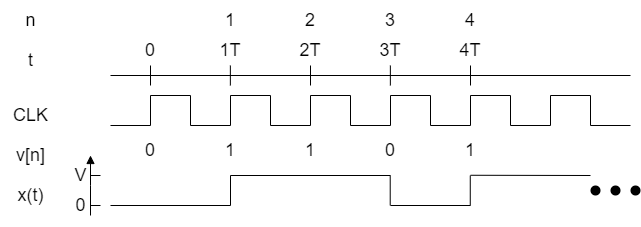
\includegraphics[scale=0.3]{./Images/01Issue/Binært signal x(t) med amplitude V.drawio.png}
	\caption{ Binært signal $x(t)$ med amplitude V og styrt av det digitale signalet $v[n]$.}
	\label{fig:binærtsignal}
\end{figure}

Det skal utarbeides en testgenerator som skal generere et tinærmet hvitt signal i det hørbareområdet. Det er spesifisert et frekvensintervall [8KHz, 9KHz] der det er spesielt viktig at støysignaleter mest mulig flatt. Utenfor dette området er det ingen spesifikke krav til signalet. Signalnivåer heller ikke spesifisert, men det skal være mulig å lytte til signalet ved hjelp av en høyttaler. I tillegg til å få optimal oppførsel i [8KHz, 9KHz] er det ønskelig at signalet “høres hvitt ut” av en person med normal hørsel som lytter på det. Tilgjengelig teknologi er en FPGA av type Lattice ICE40HX1K med de klokkefrekvenser somer mulig å stille inn ved hjelp av utviklingskortet GoBoard frå Nanland og modulen PrescalerN som finnes tilgjengelig i utviklingsverktøyet Icestudio.  Flathet måles i differansen i dB mellom høyeste og laveste verdi målt med spektrumsanalysator innen det spesifiserte frekvensområdet.
